%!TEX program = xelatex
\documentclass[aspectratio=169]{ctexbeamer}
% \usepackage{physics}  
                        %%% 宽高比说明 %%%%
%% ctexbeamer宏包支持各种宽高比,但本模板只适配了4:3(默认)和16:9的宽高比背景。
%% 添加选项aspectratio=169或aspectratio=43可以更改宽高比,默认是4:3
\usepackage[bluetheme]{ustcbeamer}
\input{ustctheme.tex}
                        %%% ustcbeamer说明 %%%%
%% 宏包使用了TikZ代码形式的背景文件(在子文件夹theme中),默认选项"bluetheme",是科大校徽的蓝色;此外ustcbeamer还内置了红色和黑色主题"redtheme","blacktheme"。

                        %%% 自定义你的主题颜色 %%%
%% 一旦使用了下述命令就会覆盖ustcbeamer的内置颜色选项,你可以设置自己喜欢的RGB色值:
% \definecolor{themecolor}{RGB}{0,150,0} % 这是绿色主题
% \definecolor{themecolor}{RGB}{0,150,150} % 青色主题,也蛮好看的

%% 注意小写rgb和大写RGB表示的色值相差255倍,即RGB{255,255,255}=rgb{1,1,1};
% \definecolor{themecolor}{rgb}{0,0.5,0.3} % 深绿色主题

%% 建议自定义的主题颜色选择偏深色
%%%%%%%%%%%%%%%%%%%%%%%%%%%%%%%%%%%%%%%%%%%%%%%%%%%%%%%%%%%%%%%%%%%%%%


\title[Ko-Sched]{
  Ko-Sched:一个离线的CUDA内核分割优化工具
}
\author[袁玉润]{报告人:袁玉润}
\institute[USTC]{
中国科学技术大学,计算机科学与技术学院
}
\date{\today}
\begin{document}
%\section<⟨mode specification⟩>[⟨short section name⟩]{⟨section name⟩}
%小于等于六个标题为恰当的标题

%--------------------
%标题页
%--------------------
\maketitleframe
%// NOTE
% 简介ko-Sched
%
%--------------------
%目录页
%--------------------
%beamer 101
% \begin{frame}%
% 	\frametitle{大纲}%
% 	\tableofcontents[hideallsubsections]%仅显示节
% 	%\tableofcontents%显示所节和子节
% \end{frame}%
%--------------------
%节目录页
%--------------------
\AtBeginSection[]{
\setbeamertemplate{footline}[footlineoff]%取消页脚
  \begin{frame}%
    \frametitle{目录}
	%\tableofcontents[currentsection,subsectionstyle=show/hide/hide]%高亮当前节,不显示子节
    \tableofcontents[currentsection,subsectionstyle=show/show/hide]%show,shaded,hide
  \end{frame}
\setbeamertemplate{footline}[footlineon]%添加页脚
}
%--------------------
%子节目录页
%--------------------
\AtBeginSubsection[]{
\setbeamertemplate{footline}[footlineoff]%取消页脚
  \begin{frame}%
    \frametitle{目录}
	%\tableofcontents[currentsection,subsectionstyle=show/hide/hide]%高亮当前节,不显示子节
    \tableofcontents[currentsection,subsectionstyle=show/shaded/hide]%show,shaded,hide
  \end{frame}
\setbeamertemplate{footline}[footlineon]%添加页脚
}

\section{研究背景}
\begin{frame}
  \frametitle{CUDA编程}
  \begin{columns}
    \begin{column}{0.4\textwidth}
      \begin{itemize}
        \item NVIDIA 并行计算架构
        \item CUDA程序包括主机(host)代码和设备(device)代码 \\
        \begin{itemize}
          \item 主机代码:运行在CPU上,负责管理设备内存,调用设备代码
          \item 设备代码(内核):运行在GPU上,负责执行计算任务
        \end{itemize}
      \end{itemize}
    \end{column}
    \begin{column}{0.60\textwidth}
      \begin{figure}
        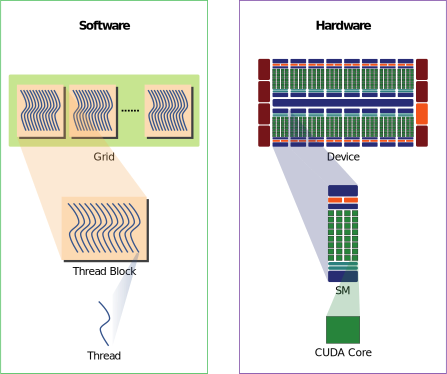
\includegraphics[width=\textwidth]{figures/programming_model_executing_model.pdf}
        % \caption{CUDA编程模型与执行模型的对应关系}
      \end{figure}
    \end{column}
  \end{columns}
\end{frame}

\begin{frame}
  \frametitle{线程块的调度策略}
  \begin{columns}
    \begin{column}{0.4\textwidth}
      \begin{itemize}
        \item 每个线程块(thread block)被分配到1个流处理器(SM)上执行
        \item 多个kernel启动后,GPU将首个kernel的线程块逐个分配给SM
        \item 若在分配完毕后设备仍有剩余硬件资源则开始分配下一个kernel
      \end{itemize}
    \end{column}
    \begin{column}{0.60\textwidth}
      \begin{figure}
        \includegraphics[width=\textwidth]{figures/kernel_nonparallel.pdf}
      \end{figure}
    \end{column}
  \end{columns}
\end{frame}

\begin{frame}
  \frametitle{内核分割}
  \begin{itemize}
    \item \textbf{问题}:若2个kernel具有不同资源瓶颈,其低并行度导致GPU资源利用率低。\\
    e.g. 计算密集型kernel与内存密集型kernel
    \begin{figure}
      \includegraphics[width=0.6\textwidth]{figures/serial_execution.drawio.pdf}
    \end{figure}
    \item \textbf{解决}:将kernel分割成多个子kernel,使得不同kernel的子内核间并行,从而实现不同kernel的并行
    \begin{figure}
      \includegraphics[width=0.6\textwidth]{figures/opt_cosched.drawio.pdf}
    \end{figure}
  \end{itemize}
\end{frame}

\begin{frame}
  \frametitle{问题}
  {\large{新问题:子内核大小的选择}}
  \begin{itemize}
    \item 子内核过大:单个子内核占用GPU资源过多,导致其他子内核无法并行执行
    \item 子内核过小:启动子内核次数较多,启动开销较大
  \end{itemize}
  \begin{figure}
    \includegraphics[width=0.7\textwidth]{figures/bad_cosched.drawio.pdf}
    \caption{\footnotesize{错误的分割方式使得 kernel 并未实现并行,反而引入了多次内核启动的开销,使得性能低于未分割内核的情况。}}
  \end{figure}
\end{frame}

\begin{frame}
  \frametitle{动机}
  \large{发现:分割参数变化时,程序性能的变化具有连续性}
  \begin{columns}
    \begin{column}{0.5\textwidth}
      \begin{flushright}
        \includegraphics[width=0.67\textwidth]{figures/consistency.drawio.pdf}
      \end{flushright}
    \end{column}
    \begin{column}{0.5\textwidth}
      图:\footnotesize{纵轴表示 vec\_add 的子内核大小,横轴表示 matrix\_mul 的子内核大小。}\\
    \footnotesize{每个坐标对应的方格颜色表示在此分割参数的组合下的程序性能,颜色越深表示性能越高。}
    \end{column}
  \end{columns}

  启发:可以类比数值计算中求解函数极值的算法(如梯度下降)来寻找性能较高的配置,而无需遍历地测试每一种可能的分割方式
\end{frame}

\section{算法设计}
\begin{frame}
  \frametitle{算法流程}
  \begin{columns}
    \begin{column}{0.5\textwidth}
      \begin{block}{}
        \indent
        \begin{enumerate}
          \item 随机选取初始子内核大小
          \item 测量当前配置的相近配置的性能
          \item 选取性能最高者为心的基准配置
          \item 重复上述操作直到基准配置优于所有相近配置
        \end{enumerate}
      \end{block}
      多次选取初始配置重复上述流程,选取最佳结果
    \end{column}
    \begin{column}{0.5\textwidth}
      \begin{figure}
        \includegraphics[width=0.9\textwidth]{figures/searching_concept.drawio.pdf}
      \end{figure}
    \end{column}
  \end{columns}
\end{frame}

\begin{frame}
  \frametitle{可变搜索步长}
  \begin{columns}
    \begin{column}{0.5\textwidth}
    \textbf{问题}
      \begin{itemize}
        \item 过小的步长会使算法收敛于局部最优解
        \item 过大的步长可能使算法在调整参数时忽略最优解
      \end{itemize}
    \textbf{解决}
      \begin{itemize}
        \item 先使用较大步长快速定位至性能高的参数区域
        \item 之后以小步长在此区域寻找精准优解
      \end{itemize}
    \end{column}
    \begin{column}{0.5\textwidth}
      \begin{figure}
        \includegraphics[width=0.9\textwidth]{figures/searching_trace_va_mm.drawio.pdf}
      \end{figure}
    \end{column}
  \end{columns}
\end{frame}

\begin{frame}
  \frametitle{分析给定分割配置下的性能}
      通过测量部分子内核的执行时间估算此配置下的完整运行时间。
      \linebreak\linebreak
      如图,启动kernel 1的1个子内核与kernel 2的5个子内核,以其执行时间的$N^1_{\text{subkernel}}$倍为完整运行时间的估算。其中$N^1_{\text{subkernel}}$为kernel 1的子内核数目。
      \begin{center}
        \includegraphics[width=0.7\textwidth]{figures/sampling.drawio.pdf}
      \end{center}
\end{frame}

\section{实验测试}
\begin{frame}
  \frametitle{实验环境}
  \begin{columns}
    \begin{column}{0.6\textwidth}
    \large{测试程序}
      \begin{description}
        \item[\texttt{matrix\_mul} (\texttt{mm})] 矩阵乘法内核
        \item[\texttt{vec\_add} (\texttt{va})] 矢量加法内核
        \item[\texttt{matrix\_transpose} (\texttt{mt})] 矩阵转置内核
        \item[\texttt{sqrt\_pow} (\texttt{sp})] 一个运算密集型内核,每个线程进行大量的平方根和指数运算。
      \end{description}
    \end{column}
    \begin{column}{0.45\textwidth}
      \large{实验涉及GPU硬件}
      \begin{itemize}
        \item NVIDIA GeForce MX250
        \item NVIDIA GeForce RTX 2080Ti
        \item NVIDIA GeForce RTX 3080
        \item NVIDIA GeForce RTX 3090
      \end{itemize}
      \ \\
    \end{column}
  \end{columns}
\end{frame}

\begin{frame}
  \frametitle{相对于未分割版本的性能}

  \begin{center}
    \includegraphics[width=0.7\textwidth]{figures/perf-eval-diff-dev.pdf}
  \end{center}

\end{frame}

\begin{frame}
  \frametitle{相对于最佳分割参数下的性能}

  \begin{center}
    \includegraphics[width=0.7\textwidth]{figures/perf-eval-compared-to-opt.pdf}
  \end{center}

\end{frame}


\begin{frame}
  \frametitle{相对于搜索时准确测量执行时间的算法的性能}

  \begin{center}
    \includegraphics[width=0.7\textwidth]{figures/perf-eval-compared-to-nonsampling.pdf}
  \end{center}

\end{frame}

\begin{frame}
  \centerline{\Large 谢谢!}
\end{frame}

\end{document}
